\section{Beam Direct Stiffness Method}

A beam element has four degrees of freedom. Two degrees of freedom at each node which includes the rotation $\theta$ and the deflection or transverse displacement, $w$.

\begin{figure}[h]	\centerline{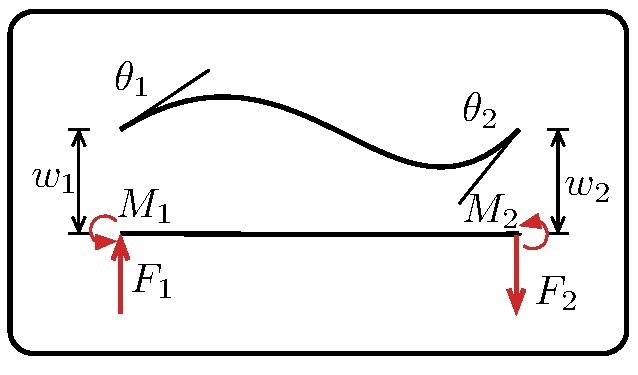
\includegraphics[width=0.7\columnwidth]{Figures/DeflectionandRotation}}
	\caption{Degrees of Freedom}
	\label{fig:DeflectionandRotation}
\end{figure}

\subsection{Bending Stiffness}

We will isolate each degree of freedom by applying boundary conditions at each node, such that each beam will only have one unrestrained kinematic unknown. Figure \ref{fig:BCFrame} shows the various boundary conditions that will be used to determine the beam bending stiffness. This will allow us to derive the force-displacement relationship necessary to solve the beam.

\begin{figure}[H]	\centerline{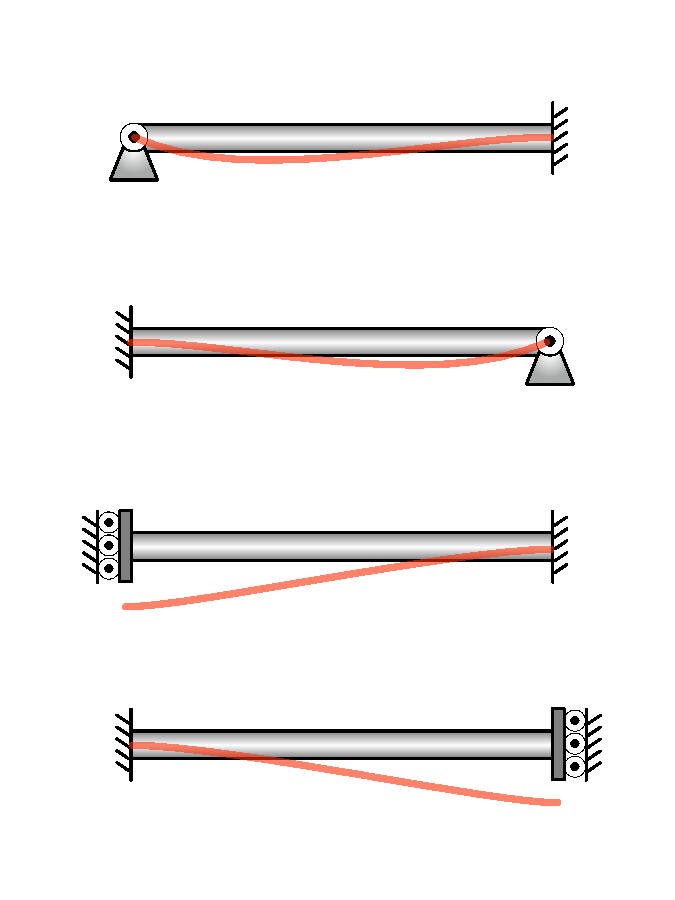
\includegraphics[width=0.9\columnwidth]{Figures/BCFrame}}
	\caption{Beam Boundary Conditions}
	\label{fig:BCFrame}
\end{figure}

\begin{align*}
	w_1=0 & \text{	} \theta_1=?\\
	w_2=0 &\text{	}  \theta_2=0
\end{align*}